\documentclass[tikz, border=5pt]{standalone}
\usetikzlibrary{arrows.meta, shapes, positioning, decorations.pathmorphing, patterns}

\tikzset{
  spring/.style = {
    decoration = {aspect=0.3, segment length=2mm, amplitude=2.5mm, coil, pre length=4mm, post length=3mm},
    decorate
  }
}

\begin{document}
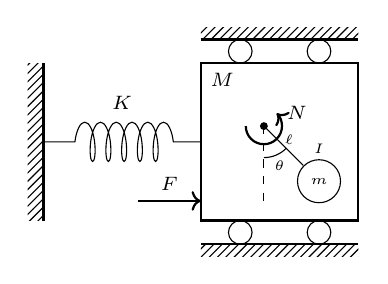
\begin{tikzpicture}

  %% TORA System

  % Wall
  \draw[thick] (-5,0) -- (-5,2);
  \fill[pattern = north east lines] (-5,0) rectangle (-5.2,2);

  % Spring
  \draw[spring] (-5,1) -- (-3,1) node[midway, above, yshift=8] {\scriptsize \(K\)};

  % Cart
  \draw[thick] (-3,0) rectangle (-1,2);
  \node[below right] at (-3, 2) {\scriptsize \(M\)};

  % Rails | bottom
  \draw[thick] (-3,-0.3) -- (-1,-0.3);
  \fill[pattern = north east lines] (-3,-0.3) rectangle (-1,-0.45);
  \draw (-2.5,-0.15) circle (0.15);
  \draw (-1.5,-0.15) circle (0.15);

  % Rails | top
  \draw[thick] (-3,2.3) -- (-1,2.3);
  \fill[pattern = north east lines] (-3,2.3) rectangle (-1,2.45);
  \draw (-2.5,2.15) circle (0.15);
  \draw (-1.5,2.15) circle (0.15);

  %% Pendulum
  \fill (-2.2,1.2) circle (0.05);
  \node[draw, circle, minimum size=0.2] (pendulum) at (-1.5,0.5) {\tiny \(m\)};
  \node[above=-0.05 of pendulum] {\tiny \(I\)};
  \draw[dashed] (-2.2,1.2) -- (-2.2,0.2);
  \draw[-] (-2.2,0.8) arc (270:315:0.4);
  \node at (-2,0.7) {\tiny \(\theta\)};
  \draw[-] (-2.2,1.2) -- (-1.5-0.2,0.5+0.2) node[midway, above, xshift=2, yshift=-3] {\tiny \(\ell\)};

  % Actuator
  \draw[->, thick] (-2.2-0.23,1.2) arc (180:405:0.23) node [right] {\scriptsize \(N\)};

  % Disturbance force
  \draw[->, thick] (-3.8,0.25) -- (-3,0.25) node[midway, above] {\scriptsize \(F\)};

\end{tikzpicture}
\end{document}
